\def\topic{Mechanization of Azriel Levy's Proof}
\ifdefined\MyHeaderIncluded
\else
\def\qwertyflag{true}

\ifdefined\MyHeaderIncluded

\else
  \newcommand{\foobar}{FooBar}
  \def\MyHeaderIncluded{true}
% if is till the end of the file

\documentclass[10pt,a4paper]{article}
\usepackage[utf8]{inputenc}
%\usepackage[german]{babel}
%\usepackage[cyrillic]{babel}
\usepackage[T1]{fontenc}
%\usepackage[T2A]{fontenc}
%\usepackage[english, russian]{babel}
\usepackage{amsmath}
\usepackage{amsfonts}
\usepackage{amssymb}
\usepackage{amsthm}
\usepackage{mathtools} %coloneqq

\usepackage{bussproofs} %

%\renewcommand{\thesubsection}{\arabic{subsection}}
%\newtheorem{thm}{Theorem}[section]
%\renewcommand{\thethm}{\arabic{subsection}.\arabic{thm}}

\usepackage{thmtools}
\usepackage{hyperref}
\hypersetup{
    colorlinks=true,
    linkcolor=blue,
    filecolor=magenta,      
    urlcolor=cyan,
    pdftitle={Overleaf Example},
    %pdfpagemode=FullScreen,
    }
%\usepackage{stix-type1}%\turnediota
\theoremstyle{definition}

\newtheorem{constructor}{Constructor}[section]
\newtheorem{iaxiom}{Axiom}
\newtheorem{axiom}{Axiom}
\newtheorem*{axiom*}{Axiom}
\newtheorem{definition}{Definition}[section]
\newtheorem*{definition*}{Definition}
\newtheorem{remark}{Remark}[section]
\newtheorem*{remark*}{Remark}
\newtheorem{recall}{Recall}[section]
\newtheorem*{recall*}{Recall}

\newtheorem{lemma}{Lemma}[section]
\newtheorem{theorem}{Theorem}[section]
\newtheorem*{theorem*}{Theorem}
\newtheorem{note}{Note}[section]
\usepackage{etoolbox}

%\newcommand*{\@Dashv}[2]{%
%  \reflectbox{$\m@th#1#2$}%
%}
\newcommand*{\separation}[3]{% 1)binder, 2)set, 3)condition
  \{#1\in #2: #3\}
}

% https://www.freecodecamp.org/news/simple-regex-tricks-for-beginners-3acb3fa257cb/
%  \\mathcal\{T\} |---> \topology
%  \\mathcal\{([^\}]*)\}   |--->  $1
\newcommand{\AND}{\ \ \&\ \ }
\newcommand{\any}{\mathrm{\ any}}
\newcommand{\borel}{\mathcal{B}}
\newcommand{\can}{\mathrm{can}}
\newcommand{\canonize}{\mathrm{canonize}}
\newcommand{\closure}{\mbox{cl}}
\newcommand{\complex}{\mathbb{C}}
\newcommand{\converges}{\longrightarrow}
\newcommand{\countable}{\mbox{\ countable}}
\newcommand{\ldefined}{\mbox{\ defined}}
\newcommand{\dom}{\mbox{dom}}
\newcommand{\Dom}{\mbox{Dom}}
\newcommand{\Done}{\noindent \textbf{Done.}\\}
\newcommand{\lexists}{\mbox{\ exists}}
\newcommand{\lforall}{\mbox{\ forall}}
\newcommand{\lunique}{\mbox{\ unique}}
\newcommand{\family}{\mathrm{\ family}}
\newcommand{\Fm}{\mathrm{Fm}}
\newcommand{\FuncSymb}{\mathrm{FuncSymb}}
\newcommand{\function}{\mathrm{\ function}}
\newcommand{\functional}{\mbox{\ functional}}
\newcommand{\IFF}{\ \Longleftrightarrow\ }
\renewcommand{\iff}{\ \longleftrightarrow\ }
\newcommand{\IMPLIES}{\ \Longrightarrow\ }
\renewcommand{\implies}{\ \longrightarrow\ }
\newcommand{\Inf}{\mathrm{Inf}}
\newcommand{\injective}{\mbox{\ injective}}
\newcommand{\injection}{\mbox{\ injection}}
\newcommand{\interior}{\mbox{int}}
\newcommand{\intersection}{\bigcap}
\newcommand{\isempty}{\mathrm{\ empty}}
\newcommand{\LB}{\mathrm{LB}}
\newcommand{\nghbset}{\mathcal{N}}
\newcommand{\nonempty}{\mathrm{\ nonempty}}
\newcommand{\Ord}{\mathrm{Ord}}
\newcommand{\power}{\mathcal{P}}
\newcommand{\pr}{\mathrm{pr}}
\newcommand{\fst}{\mathrm{fst}}
\newcommand{\snd}{\mathrm{snd}}
\newcommand{\PredSymb}{\mathrm{PredSymb}}
\newcommand{\Proof}{\noindent \textbf{Proof.}\\}
\newcommand{\ran}{\mathrm{ran}}
\newcommand{\Ran}{\mathrm{Ran}}
\newcommand{\real}{\mathbb{R}}
\newcommand{\relation}{\mathrm{\ relation}}
\newcommand{\set}{\mathrm{\ set}}
\newcommand{\singleton}{\mathrm{\ singleton}}
\newcommand{\semantics}{\mathrm{semantics}}
\newcommand{\semialgebra}{\mathcal{S}}
\newcommand{\Sup}{\mathrm{Sup}}
\newcommand{\surjective}{\mbox{\ surjective\ on\ }}
\newcommand{\Term}{\mathrm{Term}}
\newcommand{\Type}{\mathrm{Type}}
\newcommand{\topology}{\mathcal{T}}
\newcommand{\total}{\mbox{\ total\ on\ }}
\newcommand{\transitive}{\mathrm{\ transitive}}
\newcommand{\union}{\bigcup}
\newcommand{\lTrue}{\mathrm{True}}
\newcommand{\lFalse}{\mathrm{False}}
\newcommand{\lUncertain}{\mathrm{Uncertain}}
\newcommand{\lif}{\mathrm{if}}
\newcommand{\lthen}{\mathrm{then}}
\newcommand{\lelse}{\mathrm{else}}
\newcommand{\lexception}{\mathrm{exception}}
\newcommand{\lundef}{\mathrm{undef}}
\newcommand{\univocal}{\mathrm{\ univocal}}
\newcommand{\univocalat}{\mathrm{\ univocal\ at\ }}
\newcommand{\UB}{\mathrm{UB}}
\newcommand{\Un}{\mathcal{U}}
\newcommand{\Var}{\mathrm{Var}}

\newcommand{\notvarphi}{\phi}
\renewcommand{\phi}{\varphi}

\newcommand{\comment}[1]{\quad\mbox{(#1)}}
% local commands
%\preto\section{\undef\blipo} %etoolbox
\preto\subsection{\undef\blipo} %etoolbox
% https://tex.stackexchange.com/questions/105684/limit-macro-newcommand-scope-to-section
\usepackage{graphicx}
\usepackage{authblk}

\setlength\parindent{0pt} % whole doc of \noindent
\usepackage{soul}
%\usepackage{mathgl}

\fi % guard
\ifdefined\topic
\else
\def\topic{No Titel}
\fi
\title{\topic}
\author[1]{Georgy Dunaev}
\begin{document}
\maketitle
\fi
\section{Azriel Levy's union theorem}
This section cantains the expansion of Azriel Levy's article ``On Von Neumann's Axiom System for Set Theory'' \cite{Levy68}.

%This section follows the Azriel Levy's article ``On Von Neumann's Axiom System for Set Theory''(1968) availible at 
%\url{https://www.jstor.org/stable/2315201}.\\


%\ref{TakeutiZaring1982}

%(the proof needs theorems about ordinals done first)\\
\subsection{Definitions}
\iffalse
\begin{definition}[]
\label{def:}
\end{definition}
\fi

\begin{theorem}
\[
\exists T: \V \to \On  \text{ injective}
\]
\Proof
By ..., \[
\On\notin V
\]
Axiom of limitation of size:
\[
\forall C, C\in V \iff C<V
\]
Def of <:
\[
(A<B)\iffdef (\neg(B\leqslant A)),
\]
\[
(\On\notin V)\IMPLIES (\neg(\On<V))
\]
\[
\IMPLIES (\neg(\neg(V\leqslant \On)))
\]
\[
\IMPLIES (V\leqslant \On)
\]
\[
\IMPLIES (\exists T:\V\to\On\text{ injective})
\]

\Done
\end{theorem}

\iffalse
\begin{constructor}[Global order]
We have proven existence of such
\end{constructor}

Extension by new constant and function names
% https://en.wikipedia.org/wiki/Prenex_normal_form
\begin{constructor}[Henkin constructor]
For any proven(sic!) formula $\psi$ of the following form
\[
(\forall\vec{x}\exists\vec{y},\varphi),
\]
there exists a functional symbol $c_\psi$, and it's type is
\[
(\text{length}(\vec{x})\to\Term)\to\Term
\]
So the type depends a bit on the type of $\vec{x}$.
Moreover, since only for proven $\psi$ such constant can be obtained, therefore it will not be possible via constructor of the type which is independent of the value(i.e. of $\psi$).

Not necessary! We can have advanced axiom! (premise is the stat)
I.e. there is a default value, e.g. the empty set, in case if $\psi$ is not a valid formula.
\end{constructor}
\begin{notation}
\[
\const:\Fm\to\Term
\]
\end{notation}
\fi

\begin{constructor}[Henkin constructor]\ \\%new
%For any formula $\psi$ "of the following form"(this is BAD!)
%\[
%(\forall\vec{x}\exists\vec{y},\varphi),
%\]
%there exists a functional symbol $c_\psi$, and it's type is
%\[
%(\text{length}(\vec{x})\to\Term)\to\Term
%\]
\iffalse
For any formula $\varphi$, for any list of variables $\vec{x}$ and $\vec{y}$,
there exists a functional symbol $f_\psi$, where
\[
\psi\ceq(\forall\vec{x}\exists\vec{y},\varphi).
\].

\fi
For any bounded by term formula $\kappa$, $c_{\kappa}$ is a term.
\[
h:\BoundFm\to\Term
\]
\[
\kappa \mapsto h_\kappa
\]
\end{constructor}

\begin{axiom}[Henkin axiom schema]\ \\
\label{ax:Henkin}
\iffalse
variant1:
\[
(\forall\vec{x}\exists y,\varphi)
\implies
(\forall\vec{x}\varphi[f(\vec{x})/y])
\]
variant2:
\fi
\[
(\exists y.\varphi)
\implies
(\varphi[h_{(y.\varphi)}/y])
\]
\iffalse
%GOOD, BUT UGLY
\[
(\exists \kappa)
\implies
(\varphi[h_\kappa/\fst(\kappa)])
\]
\[
(\exists (y.\varphi))
\implies
((y.\varphi)(h_{(y.\varphi)}))
\]
\fi

\[
\FV(c_{(y.\varphi)}):=\FV((y.\varphi))
\]
Semantics: if the assumption is true, then $c_{(y.\varphi)}$ is one of such objects $y$, that $\varphi$ holds(in our case classes are objects);  if the assumption is not true, then $c_{(y.\varphi)}$ is interpreted as some default class. The empty class is chosen to be default. Note, that the implementation of the interpretation of this symbol may require meta-theoretical choice on the domain (i.e. on the conglomerate of all classes) as well, or something like that.
\end{axiom}

\begin{definition}[Global choice, variant 1]\ \\
If $x\notin \FV(S)$ then
\[
c(S)\ceq h_{(x.(x\in S))}
\]
\end{definition}
\iffalse
\begin{definition}[meta-definition]
\[
\text{T} \eqdef h_{(T.(T:\V\to\On\text{ injective}))}.
\]

%Let $\text{T}$ be a new constant, ...

Choose once any $T$, such that $T:\V\to\On\text{ injective}$,
\[
\text{T}:=T.
\]
\[
\text{T}:\V\to\On\text{ injective}.
\]
\end{definition}
\fi
\begin{lemma}
\[
(\exists T:B\to C\text{ injective})
\implies 
(
(\exists F:C\to B\text{ surjective})
\lor
(B=\emptyclass)
)
\]
\Proof
\[
F\ceq G^\top\cup((C\setminus T[B])\times\{b\})
\]
\Done
\end{lemma}

\begin{lemma}[there exist an indexing of set with ordinal numbers]
\label{lem:exOnToVSurj}
\[
\exists F:\On \to \V \text{ surjective}
\]
\Proof
It follows from the previous lemma for $C\ceq\On$, %bad:$T\ceq\text{T}$,
 $B\ceq\V$, that
\[
(\exists T:\V\to \On\text{ injective})
\implies 
(
(\exists F:\On\to \V\text{ surjective})
\lor
(\V=\emptyclass)
)
\]
From the axiom of existence of a set, it follows that $(\V\neq\emptyclass)$.\\
From this fact and the theorem 1.1, it follows, that
\[
(\exists F:\On\to \V\text{ surjective})
\]
\Done
\end{lemma}


\begin{definition}[well-ordering of universal class]\ \\
\label{def:FwoV}
\iffalse
Choose once any $F$, such that $\On \to \V \text{ surjective}$,
\[
\text{F}:=F.
\]
\[
\text{F}:\On \to \V \text{ surjective}
\]
\fi
\[
\F\eqdef h_{(F.(F:\On \to \V \text{ surjective}))}
\]
\end{definition}
Obviously, from the lemma \ref{lem:exOnToVSurj} and the axiom \ref{ax:Henkin}, it follows that
\[
\F:\On \to \V \text{ surjective}.
\]


\begin{definition}[the ``minimal'' section of $F$ which returns minimal ordinals]
\label{def:Gsect}
%G_F(y)\eqdef\inf\cc{x\in\On}{F(x)=y}
\[
\G(y)\eqdef\inf\cc{x\in\On}{\F(x)=y}
\]
\end{definition}

\begin{definition}[global choice]\ \\%, variant 2
Here we define a functional symbol $c$ as an alias for some bound term:
\[
c(S) :\equiv \F(\inf \G[S])
\]
\iffalse
GOOD BUT WEIRD
Assume $(S\neq\emptyclass)$.
\[
c(S)\eqdef F(\inf G_F[S])
\]
\[
c(S)\eqdef F(\inf T[S])
\]
\fi
\end{definition}

\begin{lemma}[global choice chooses]
\label{lem:j}
\[
(S\neq\emptyclass)\implies(c(S)\in S)
\]
\Proof
\[
(S\subclass \V)
\LAND
(\G : V\to \On)
\IMPLIES
(\G[S]\subclass\On)
\]
\[
(S\neq\emptyclass)
\LAND
(S\subclass \V)
\LAND
(\G : V\to \On \text{ surjective})
\IMPLIES
(G[S]\neq\emptyclass)
\]
Since $(\G[S]\subclass\On)$ and $(G[S]\neq\emptyclass)$, then $((\G[S]\intersection \On)\neq\emptyclass)$.\\
Therefore, by theorem \ref{thm:infordmin}, $(\inf(\G[S])\in \G[S])$
\Done
\end{lemma}


\begin{definition}[tilde]
\label{def:tilde}
\[
\tilde{f}\eqdef
\begin{cases}
    f,& \text{if }f\text{ is a function},\\
    \emptyclass,& \text{otherwise}.
\end{cases}
\]
\end{definition}
%\[
%\ev_\cdot:X\to((X\to Y)\to Y),
%\]
%\[
%\ev_x(f)\ceq f(x).
%\]
\begin{definition}[evaluation class-function]\ \\
\label{def:evclass}
Implying that $f(x)=\emptyclass$ in case of $x\notin\dom(f)$,
\[
\ev_x\eqdef\cc{(f,f(x))}{f\in\V}
\]
\end{definition}
\begin{definition}[R function]
\label{def:Rfunc}
\[
R\eqdef((\tilde{\cdot})\circ F)
\]
\end{definition}
\begin{definition}[Q(x)]
\label{def:Qx}
\[
Q(x)\eqdef\ev_x[R[x]]
\]
\end{definition}

\begin{definition}[h function]
\label{def:hfunc}
\[
h(x)\eqdef\inf(\On\setminus(Q(x)))
\]
\end{definition}
\begin{definition}[beta]
\label{def:beta}
\[
\beta\eqdef G(h)
\]
\end{definition}
\begin{definition}[bounded subclasses of On]\ \\
\label{def:bddscOn}
In context of $(b\subclass\On)$,
\[
(b\text{ bounded})\iffdef(\exists \beta\in\On:b\subclass\beta)
\]
\[
(b\text{ unbounded})\iffdef(\neg(b\text{ bounded}))
\]
\end{definition}
\subsection{Sets of ordinals are bounded}
\begin{lemma}[subsets of On are bounded]
\label{lem:ssOnBdd}
\[
(b\set)\land(b\subclass\On)\implies(b\text{ bounded})
\]
\Proof
Step 1:
\[
(x\set)
\IMPLIES
(Q(x)\set)
\]
\[
(Q(x)\set)
\IMPLIES
((\On\setminus Q(x))\neq\emptyclass)
\]
\[
\IMPLIES
\inf(\On\setminus Q(x)) \in (\On\setminus Q(x))
\]
\[
\IMPLIES
h(x)\in (\On\setminus Q(x))
\]
\[
\IMPLIES
(h(x)\in \On)
\land
(h(x)\notin Q(x))
\]
Step 2:
\[
(y\set)
\LAND
(F:\On\to\V\text{ surjective})
\IMPLIES
F^\top[\{y\}]\neq\emptyclass
\]
\[
\IMPLIES
\inf(F^\top[\{y\}])\in F^\top[\{y\}]
\]
\[
\IMPLIES
G(y)\in F^\top[\{y\}]
\]
\[
\IMPLIES
(G(y)\in\On)\land( F(G(y))=y)
\]
\Done
\end{lemma}

\subsection{Union of a set is a set}
\begin{lemma}[techlem]
\label{lem:techlem}
\[
F[\alpha]\supseteq \union a
\]
\Proof
Fix $\left(b\in\union a\right)$. To show: $n\in F[\alpha]$.
\[
\left(b\in\union a\right)
\IMPLIES
\exists b\in a:n\in b.
\]
Due to lemma \ref{lem:ssOnBdd} $H(b)$ is a strict upper bound of $G[b]$.
\[
(b\set)
\IMPLIES
(G[b]\in\power(\On))
\]
\[
\IMPLIES
(G[b]\text{ is bounded})
\]
There is a bound, therefore, there is a strict bound.
\[
(a\set)
\LAND
(H\text{ class-function})
\implies
(H[a]\set)
\]
\[
(H[a]\set)
\LAND
(H[a]\subclass\On)
\IMPLIES
(\exists \alpha\in\On:H[a]\subclass\alpha)
\]
\[
(b\in a)
\IMPLIES
(H(b)\in H[a])
\]
\[
H[a]\subclass\alpha
\IMPLIES
H(b)\in\alpha
\]
\[
H(b)\in\alpha
\IMPLIES
H(b)\subsetneq\alpha
\]
\[
G[b]\subclass H(b)
\LAND
H(b)\subsetneq\alpha
\IMPLIES
G[b]\subclass\alpha
\]
\[
\IMPLIES
(F[G[b]]\subclass F[\alpha])
\]
\[
F[G[b]]=b
\]
\[
b\subclass F[G[b]]
\LAND
(F[G[b]]\subclass F[\alpha])
\IMPLIES
(b\subclass F[\alpha])
\]
\[
(n\in b)
\LAND
(b\subclass F[\alpha])
\IMPLIES
(n\in F[\alpha])
\]
\Done
\end{lemma}

\begin{theorem}[union of set is a set]
\label{thm:unionisset}
\[
(A\set)
\implies
\left(\union A\set\right)
\]
\Proof
\[
H(b)\eqdef\inf\cc{e}{e\text{ strict upper bound of }G[b]}
\]
\[
(a\set)
\LAND
(H\text{ class-function})
\implies
(H[a]\set)
\]
\[
(H[a]\set)
\LAND
(H[a]\subclass\On)
\IMPLIES
(H[a]\in\power(\On))
\]
\[
(H[a]\in\power(\On))
\IMPLIES
(\exists\alpha\in\On:H[a]\subclass\alpha)
\]
\[
(\alpha\set)
\LAND
(F\text{ class-function})
\IMPLIES
(F[\alpha]\set)
\]
Statement of the lemma \ref{lem:techlem}: $F[\alpha]\supseteq \union a$.
\[
(F[\alpha]\set)
\LAND
\left(\left(\union a\right)\subclass \left(F[\alpha]\right)\right)
\IMPLIES
\left(\left(\union a\right)\set\right)
\]
\Done
\end{theorem}
\iffalse
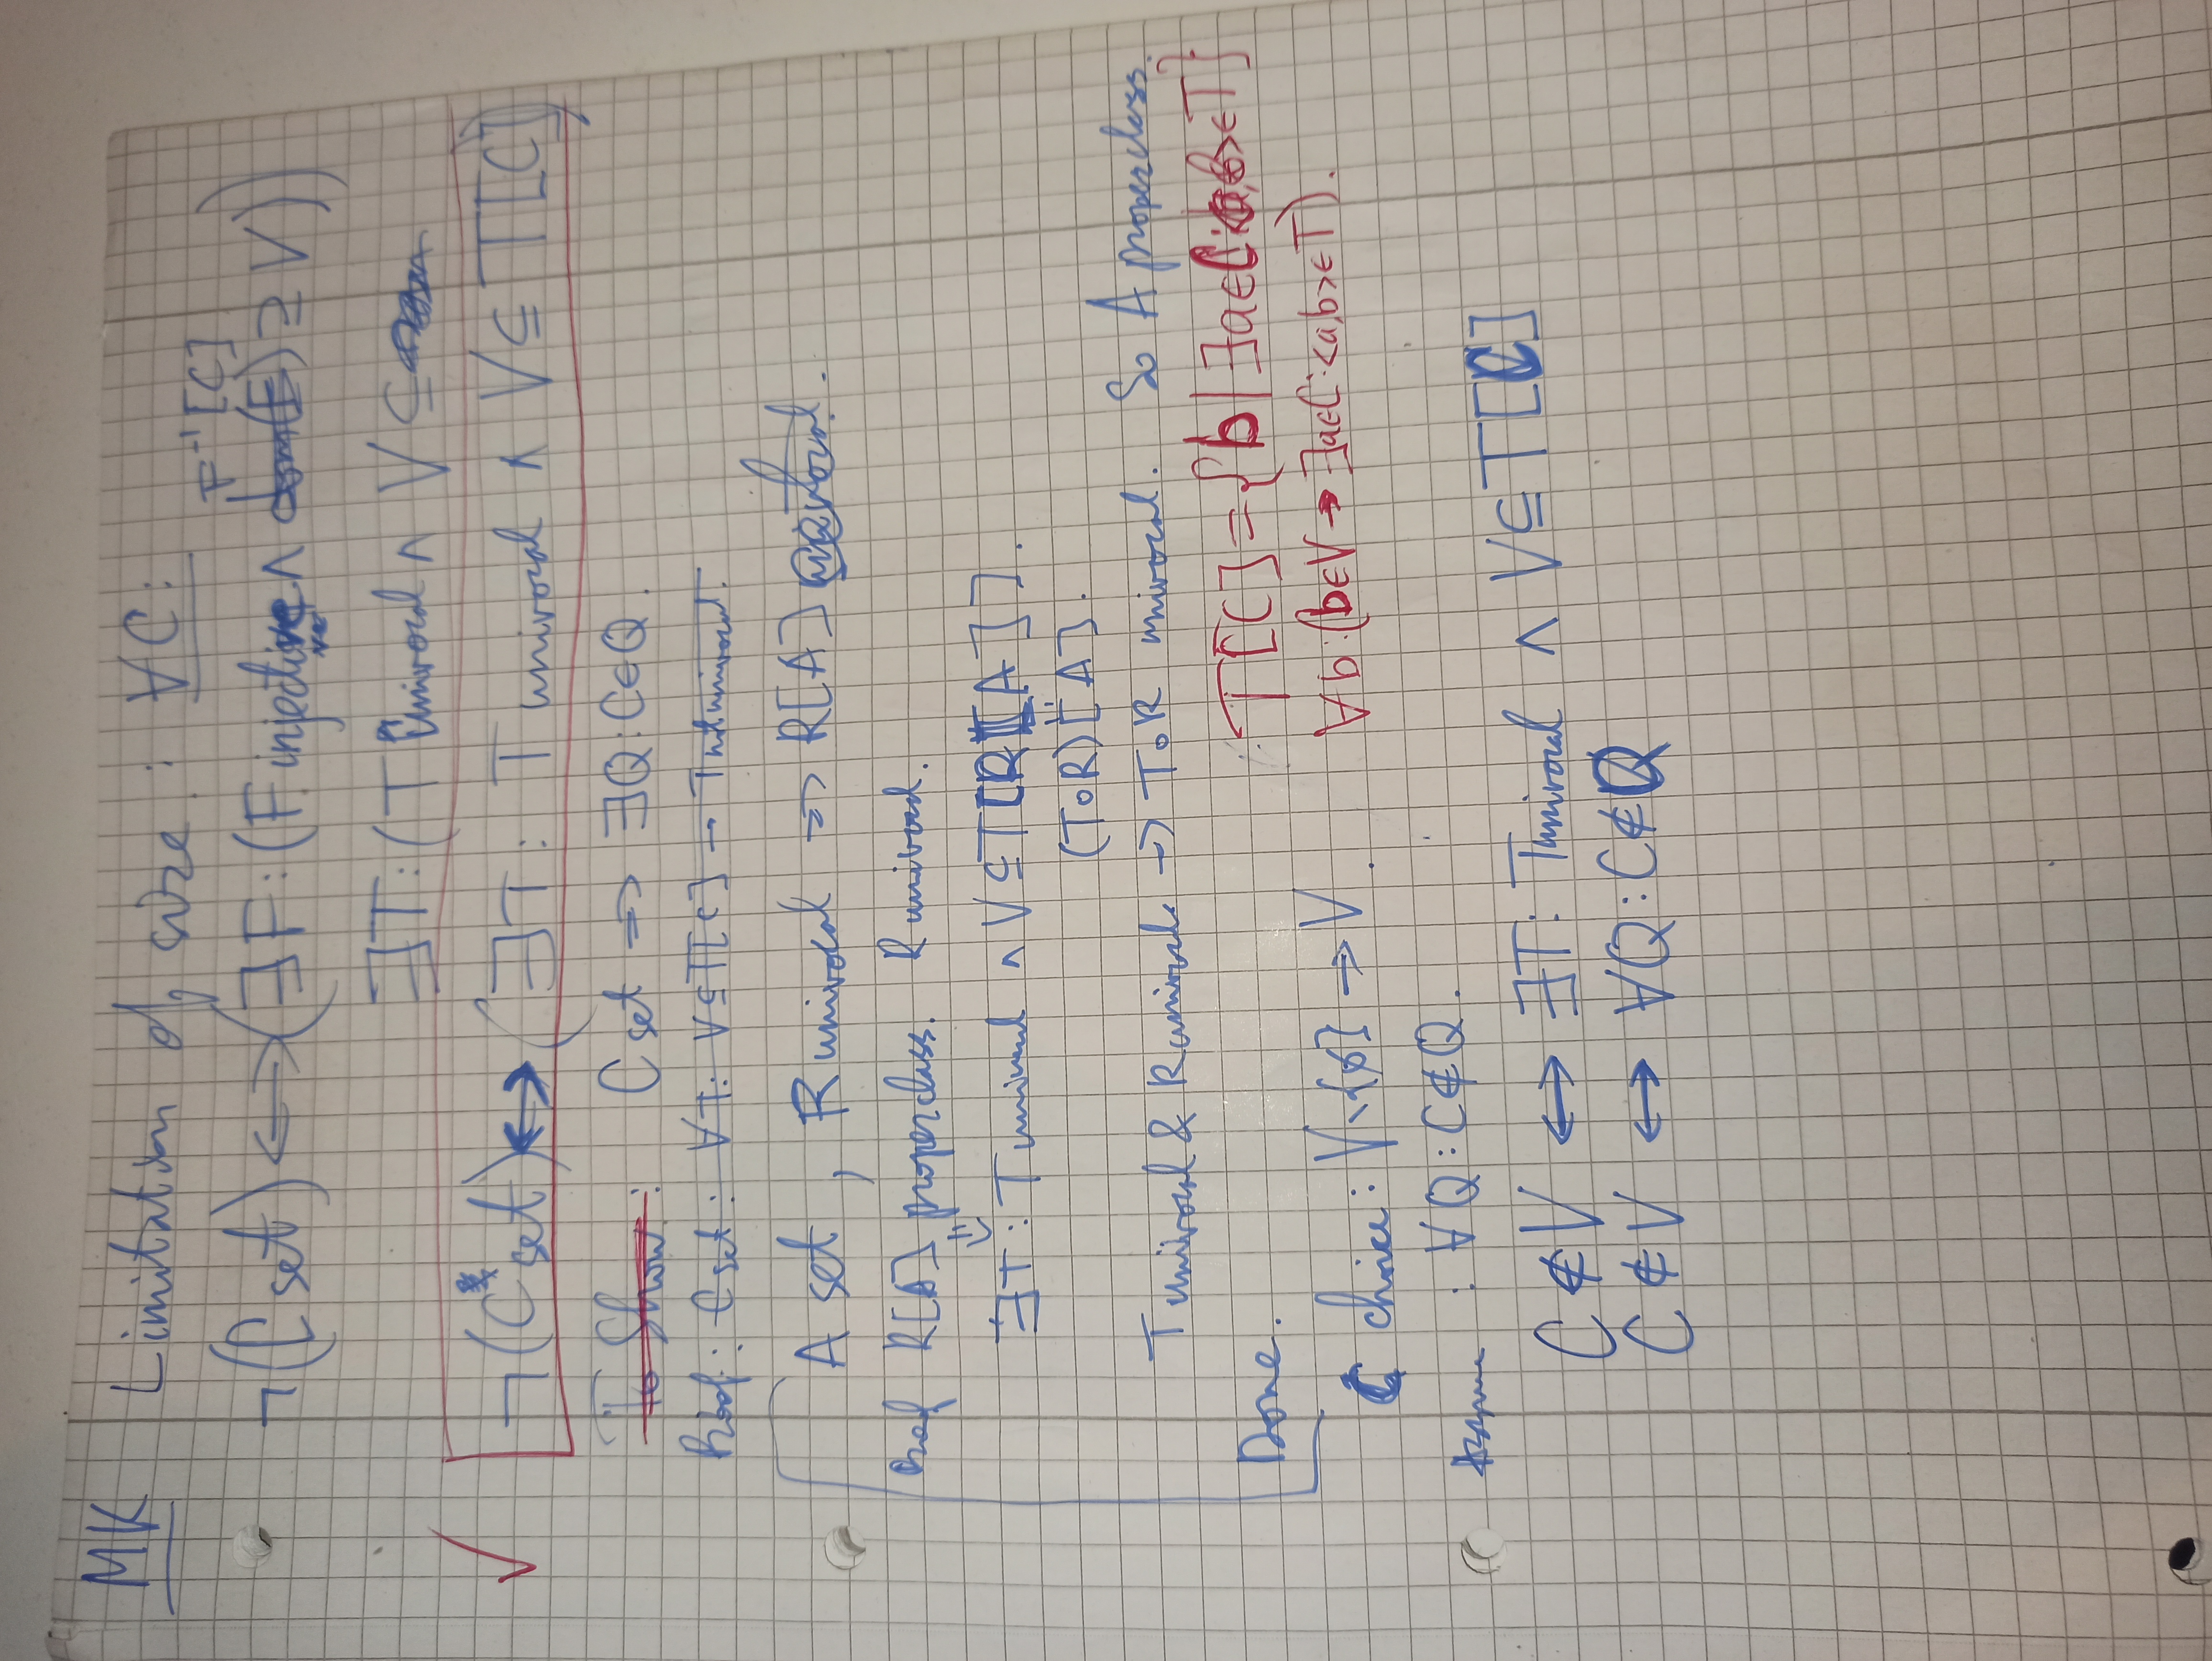
\includegraphics[angle=-90,origin=c,scale=0.1]{azriel_levy/1.jpg}\\
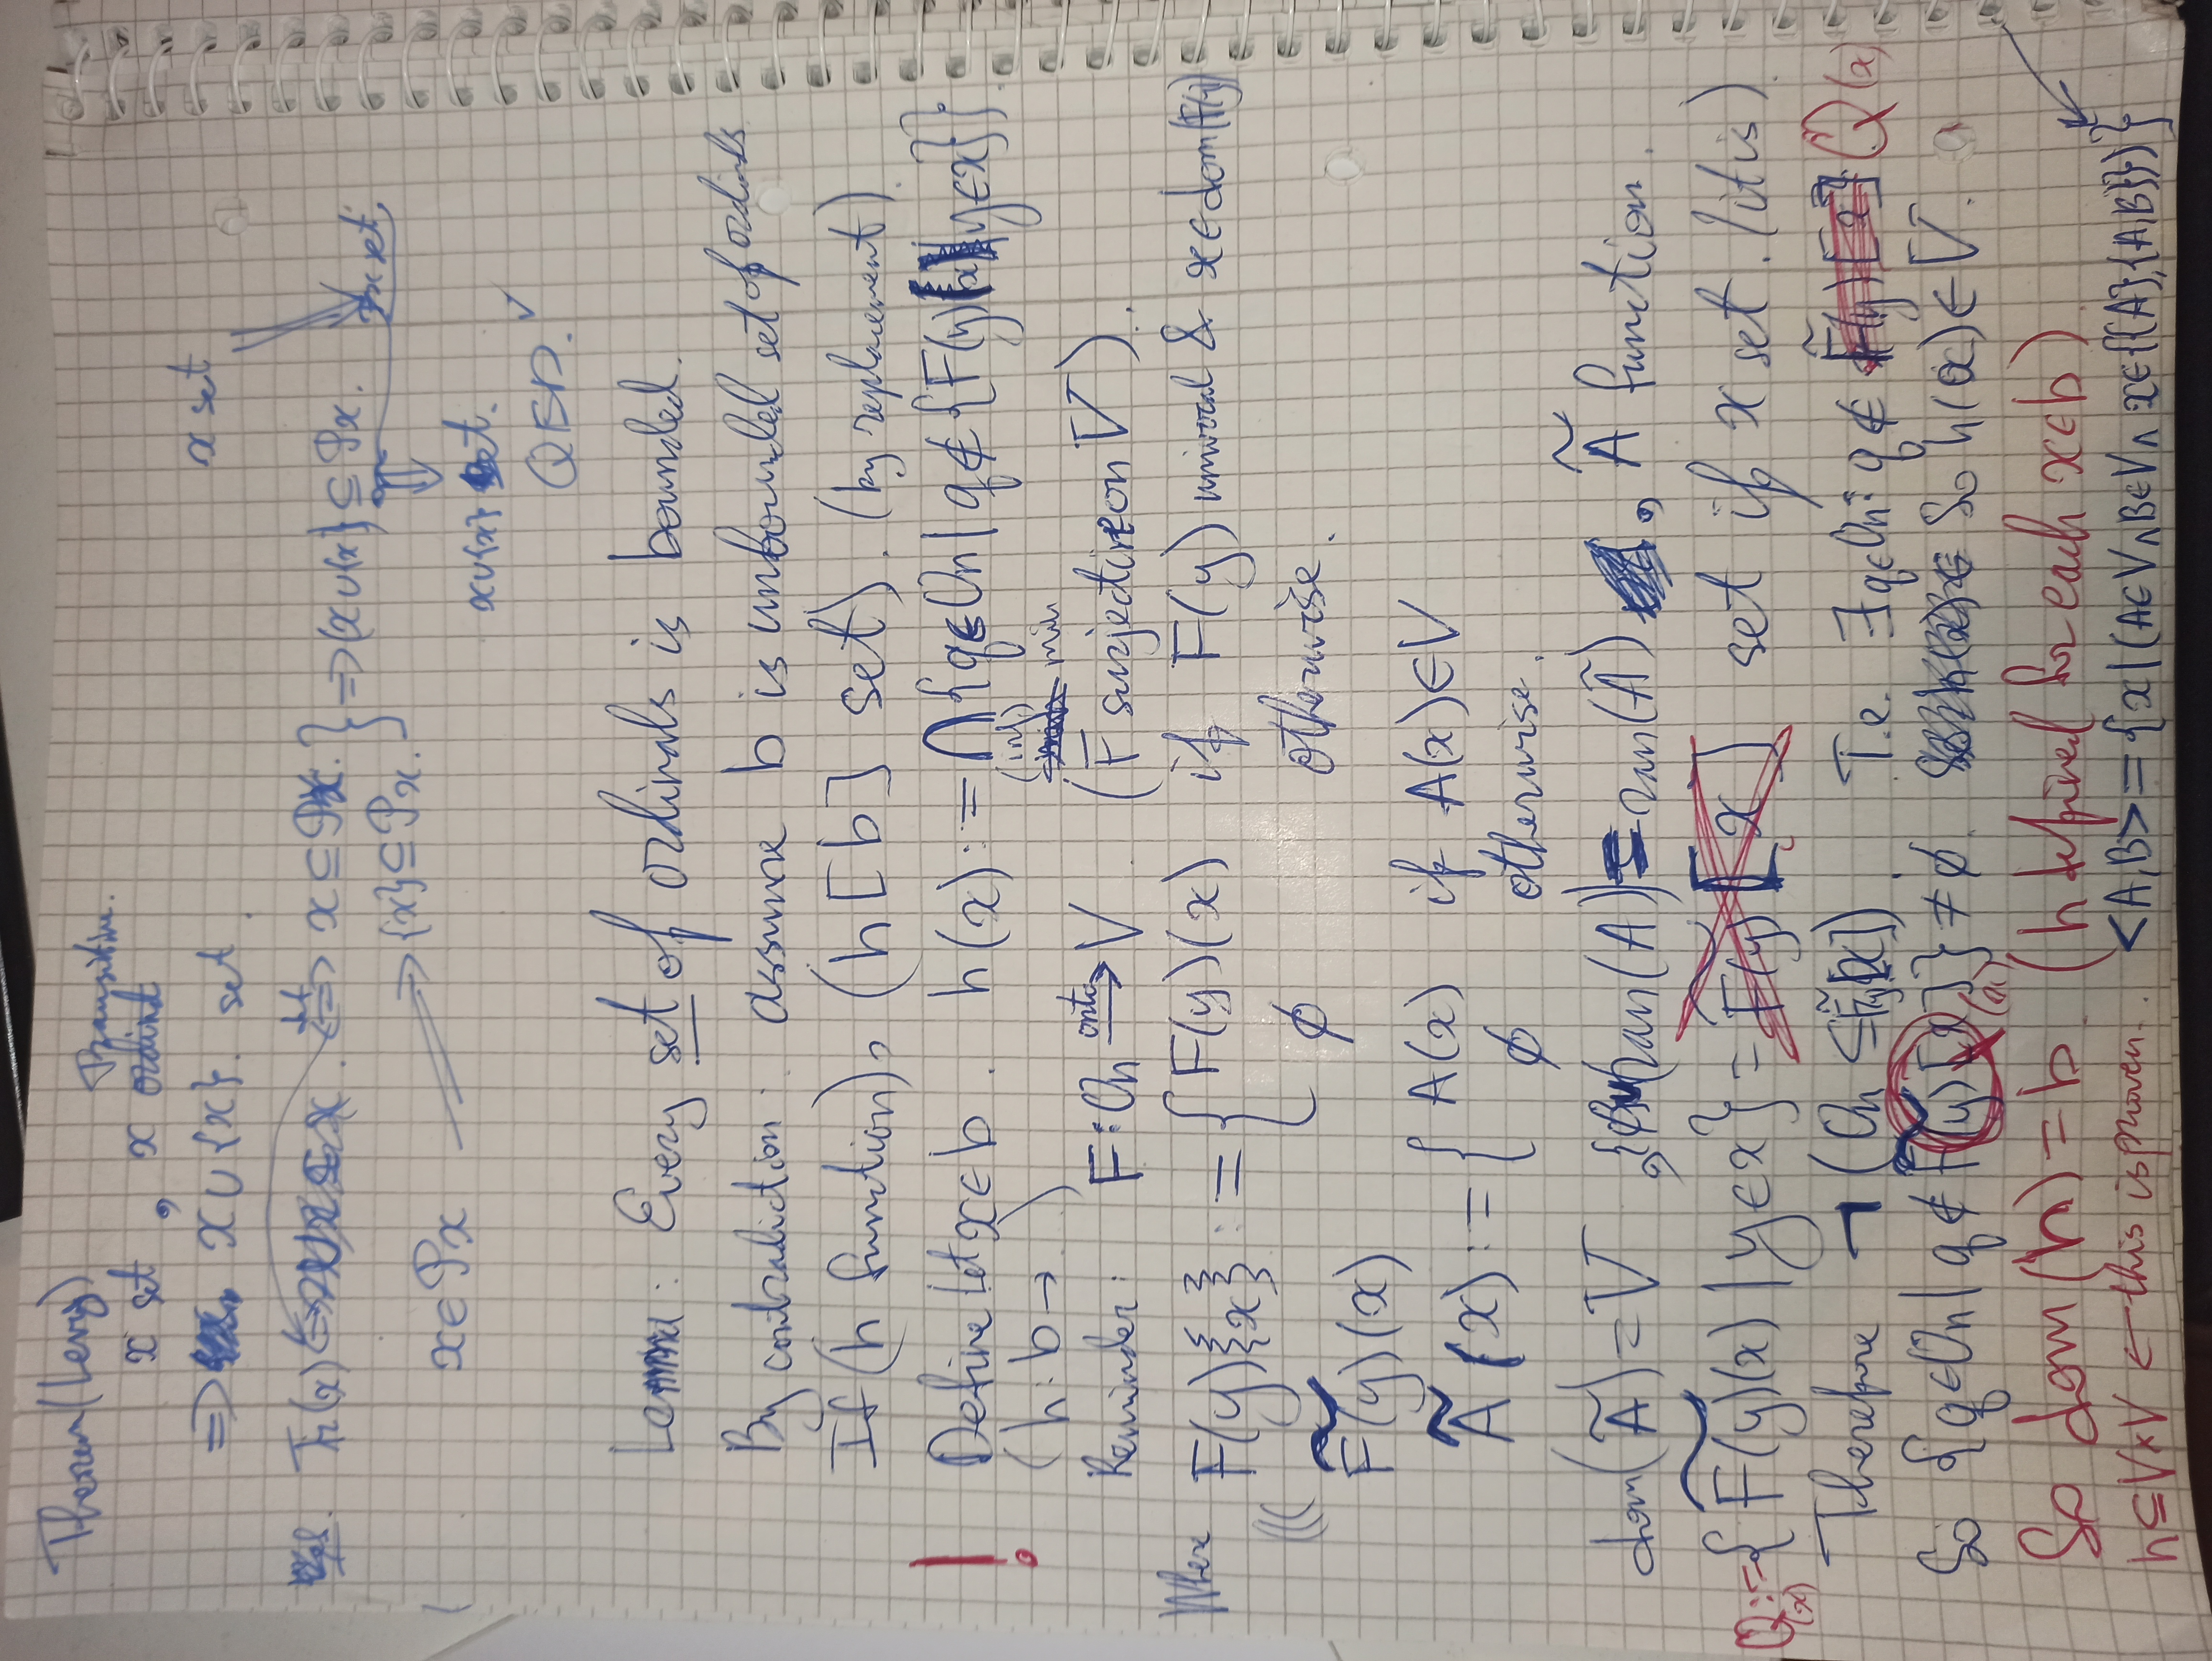
\includegraphics[angle=-90,origin=c,scale=0.1]{azriel_levy/2.jpg}\\
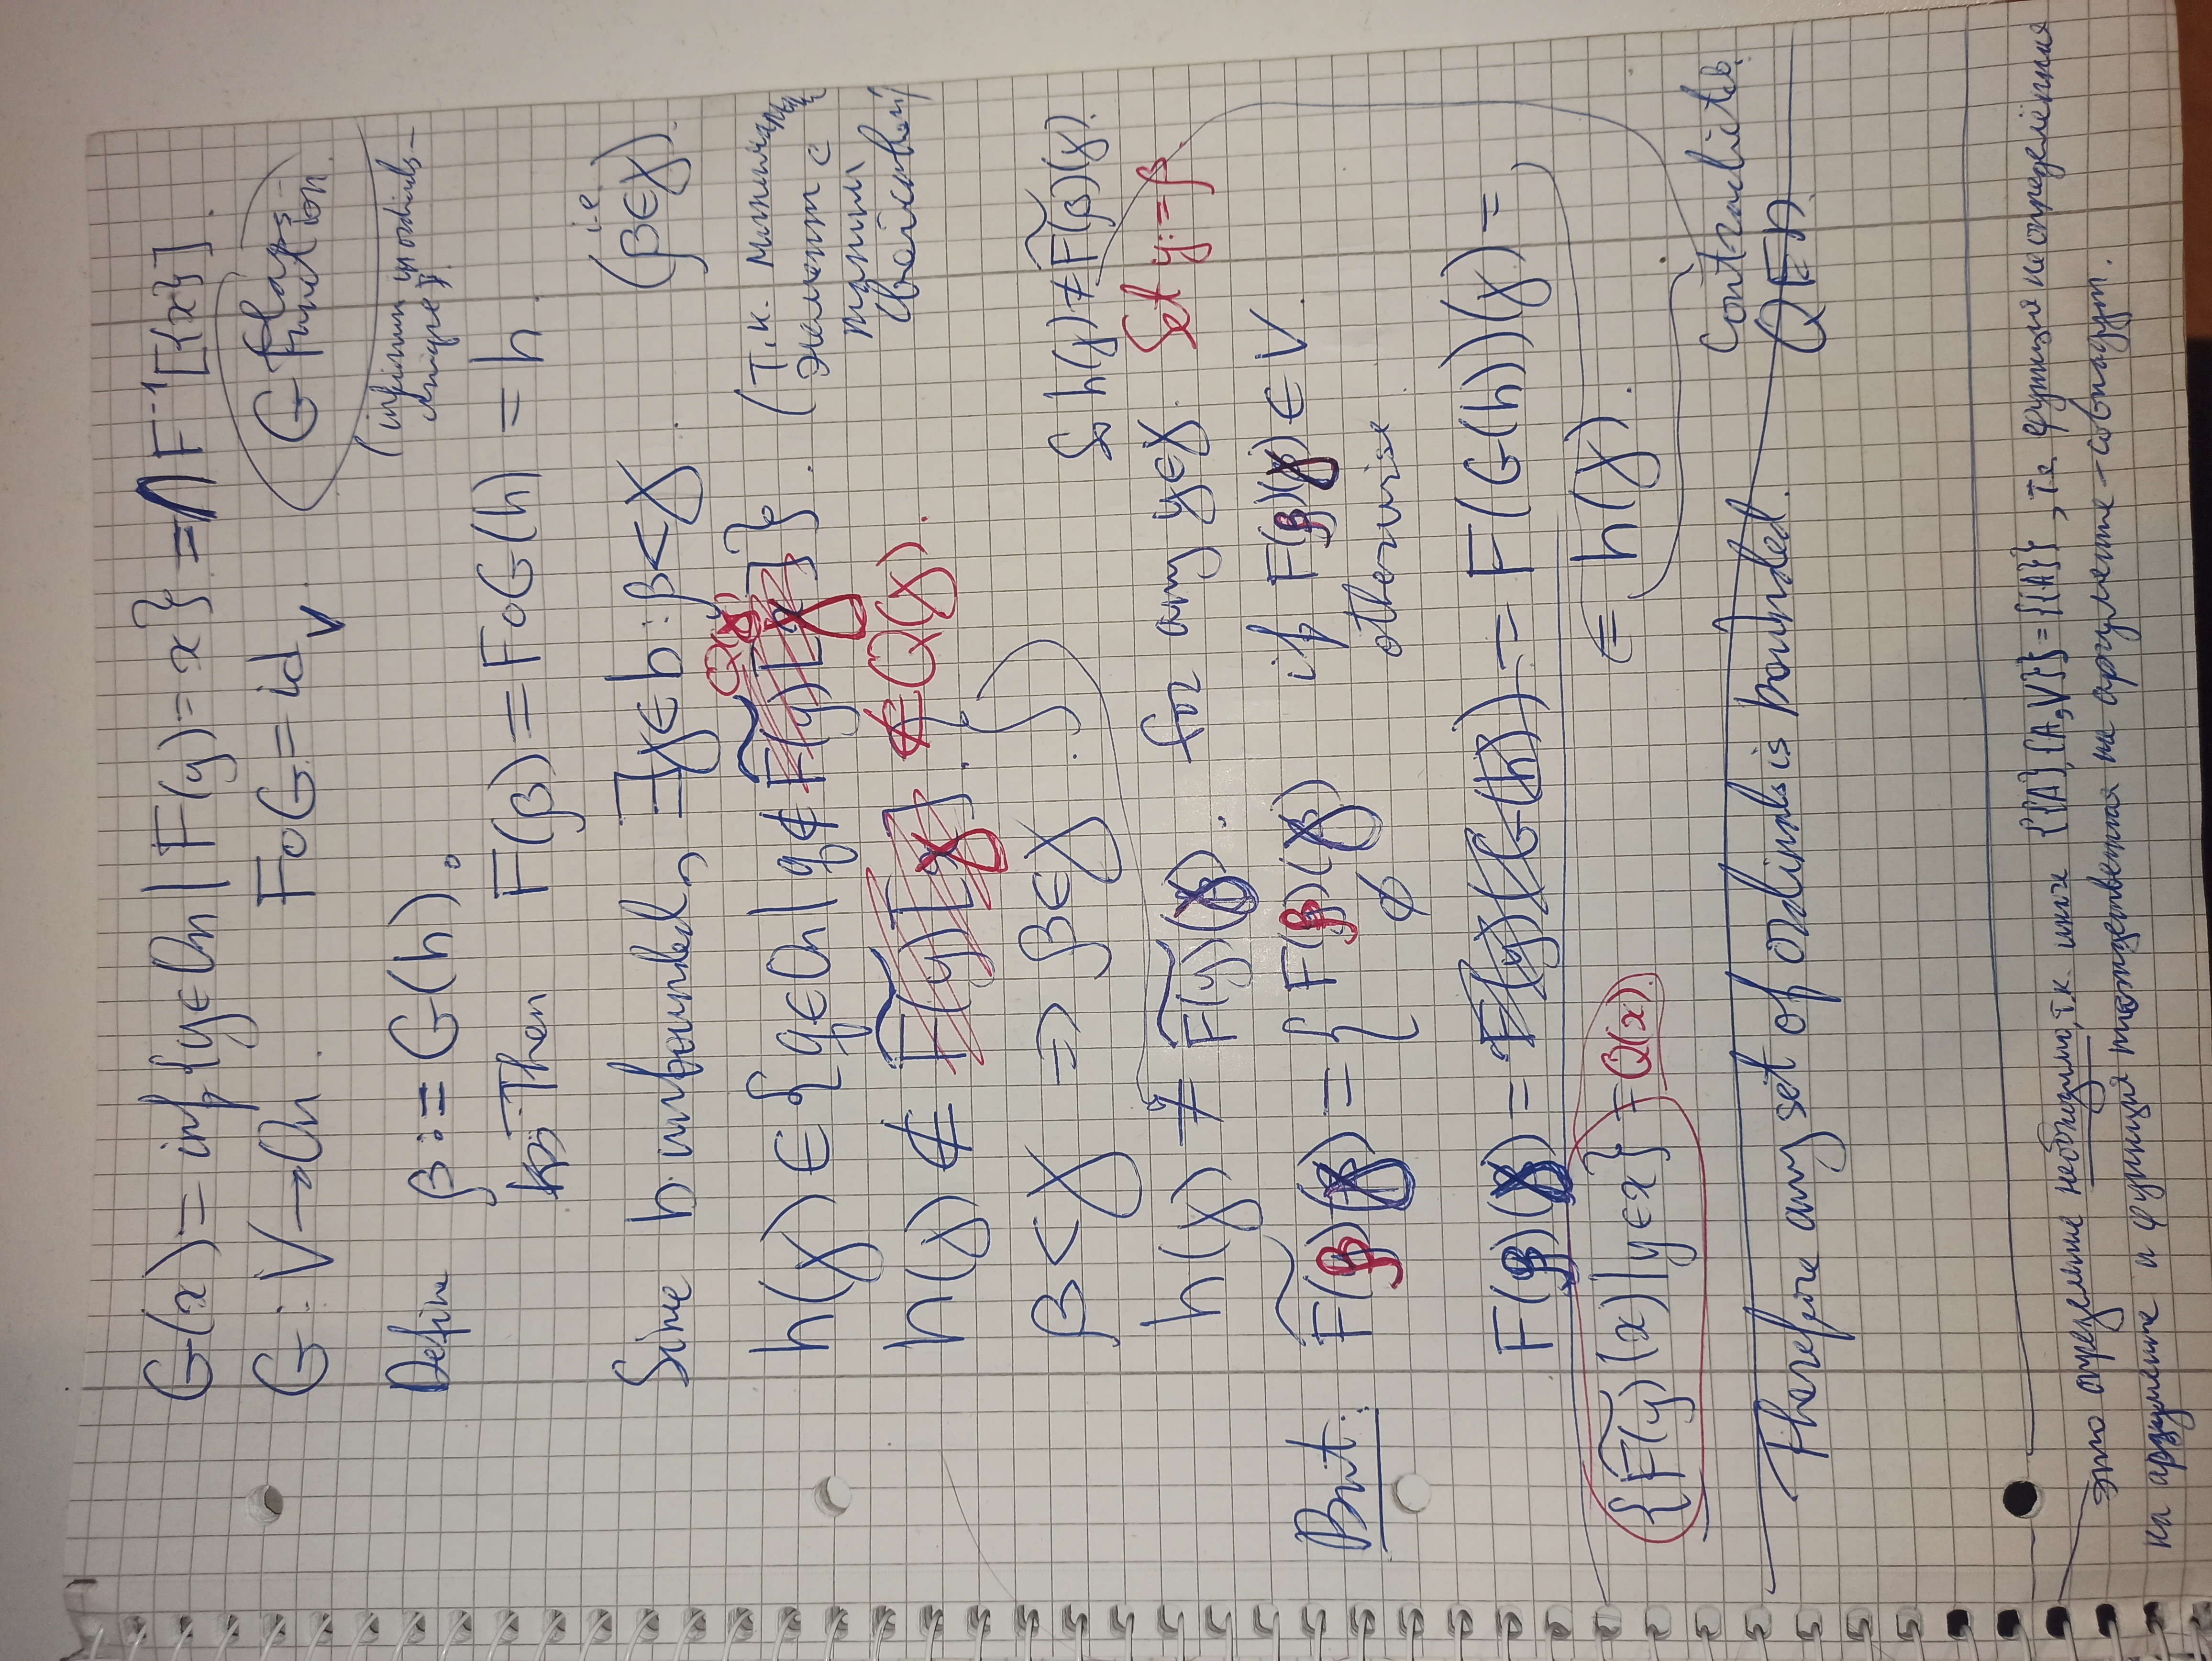
\includegraphics[angle=-90,origin=c,scale=0.1]{azriel_levy/3.jpg}\\
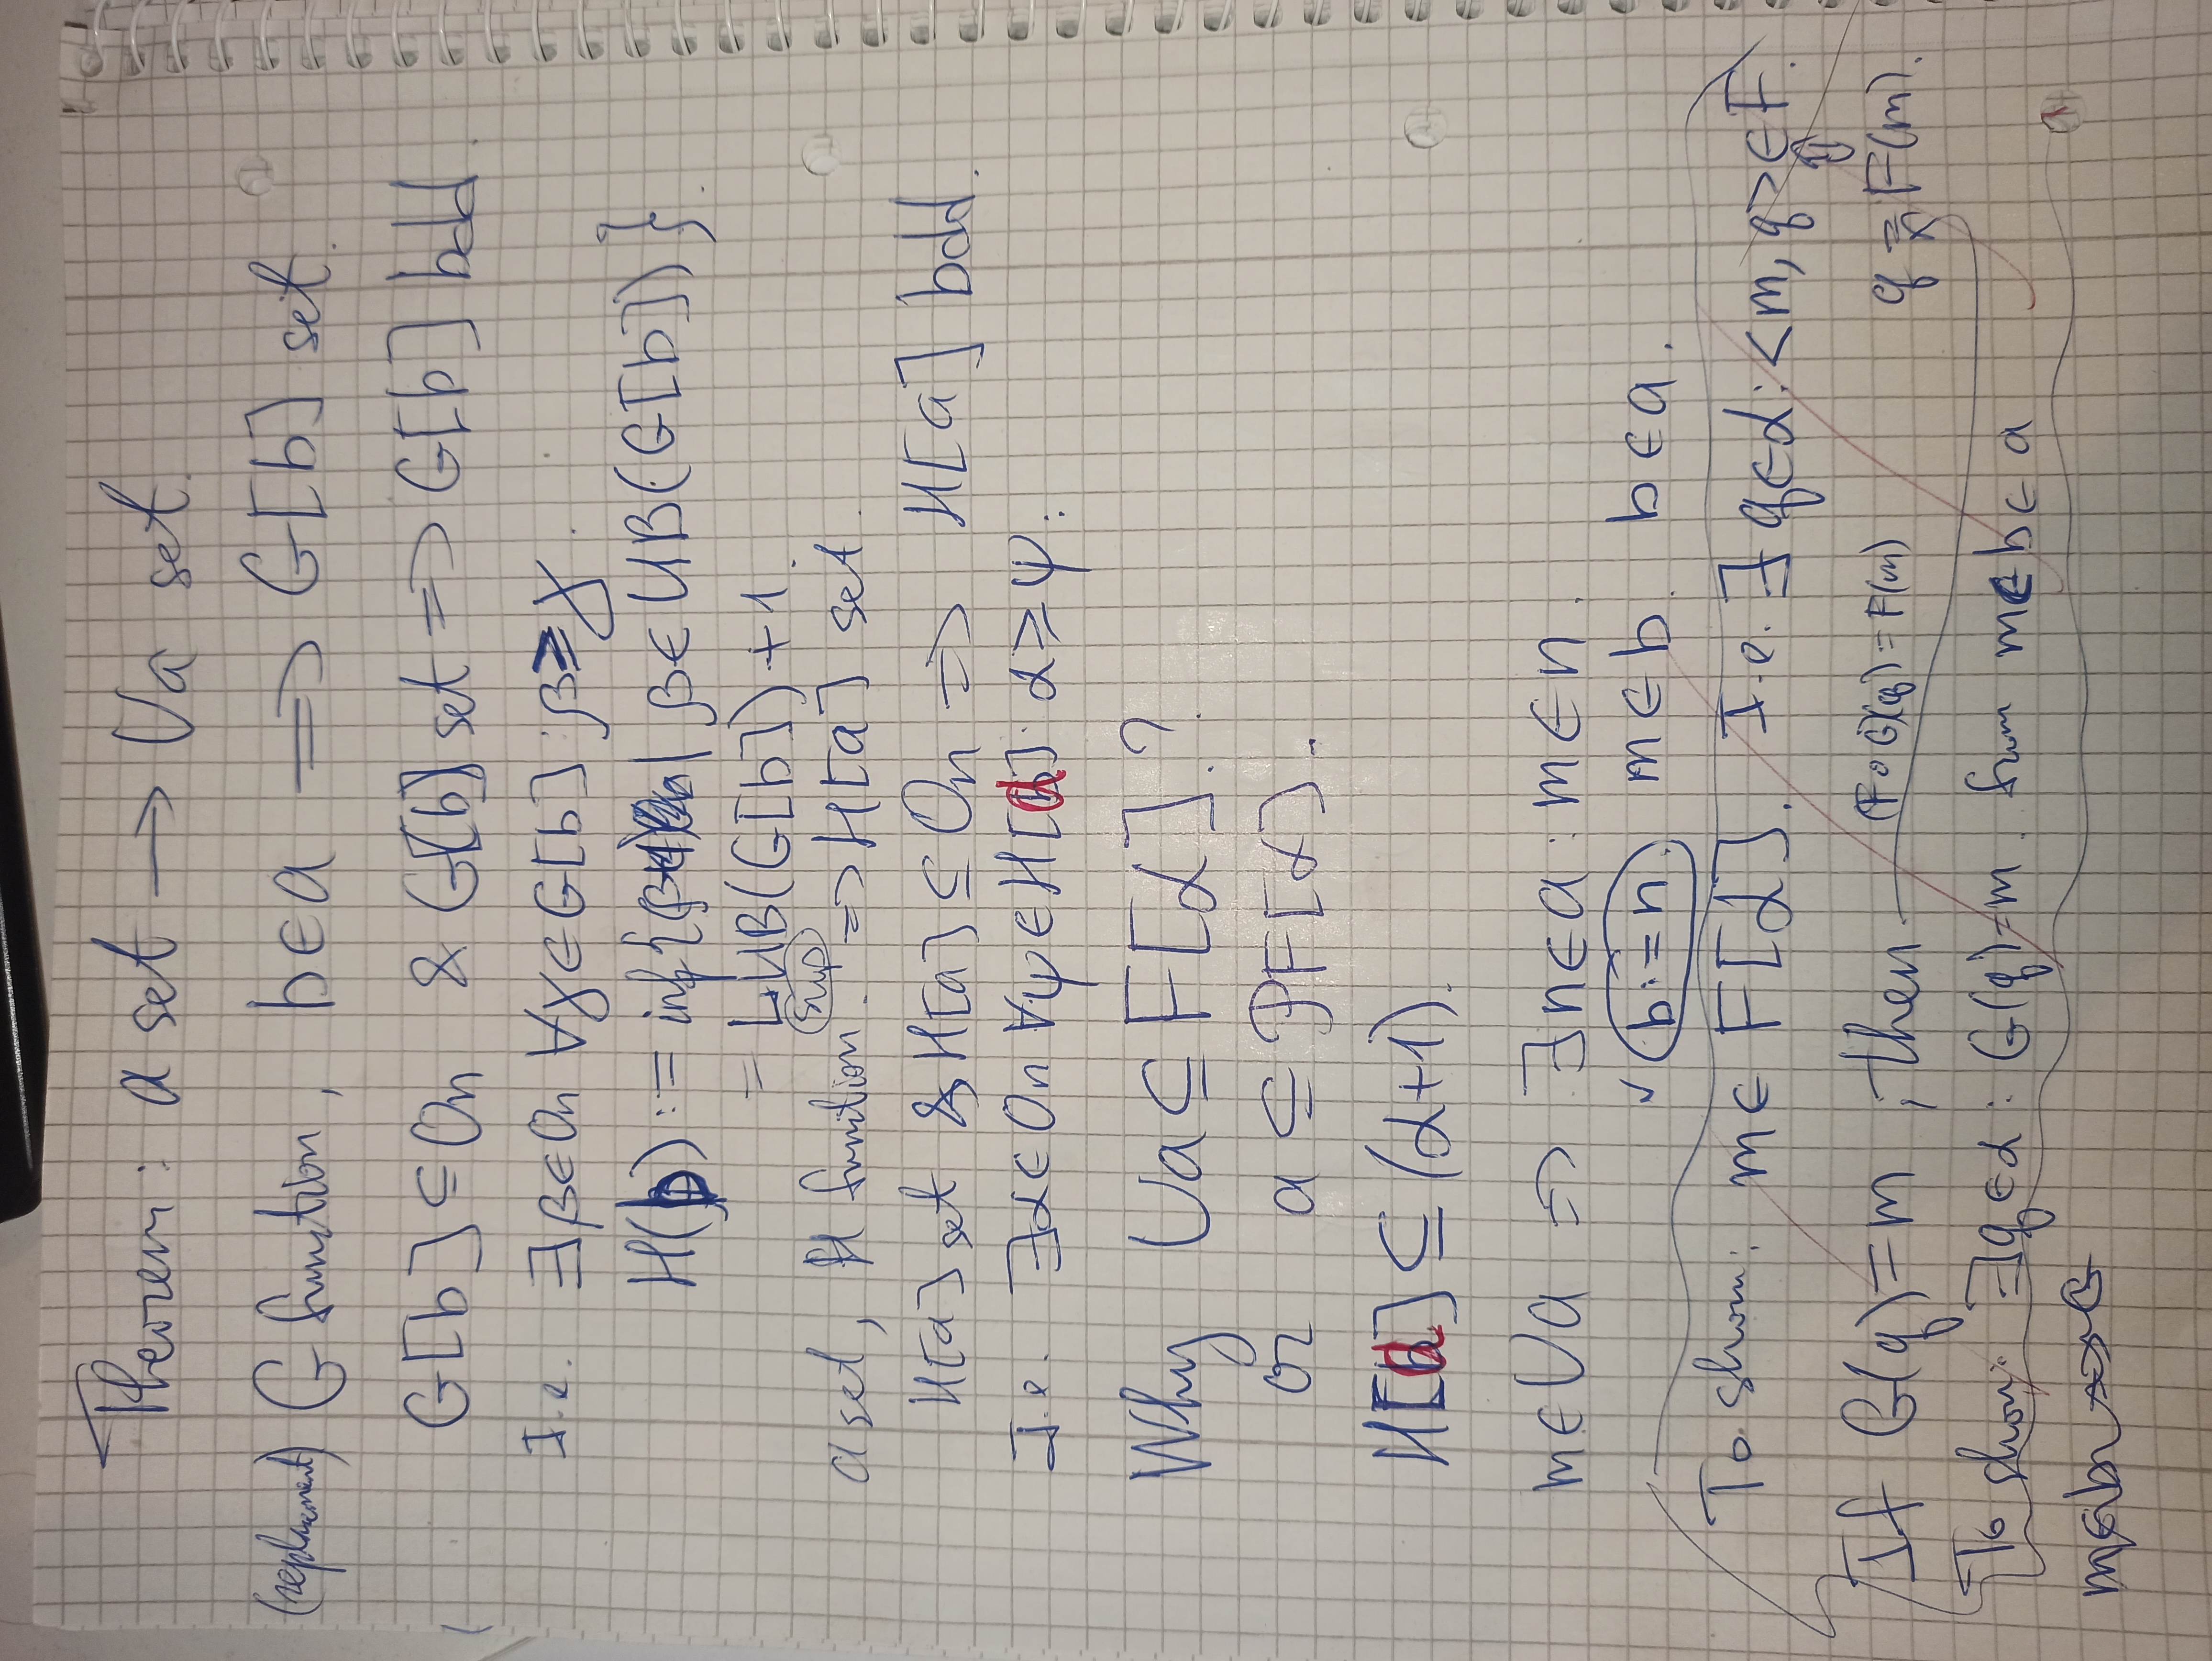
\includegraphics[angle=-90,origin=c,scale=0.1]{azriel_levy/4.jpg}\\
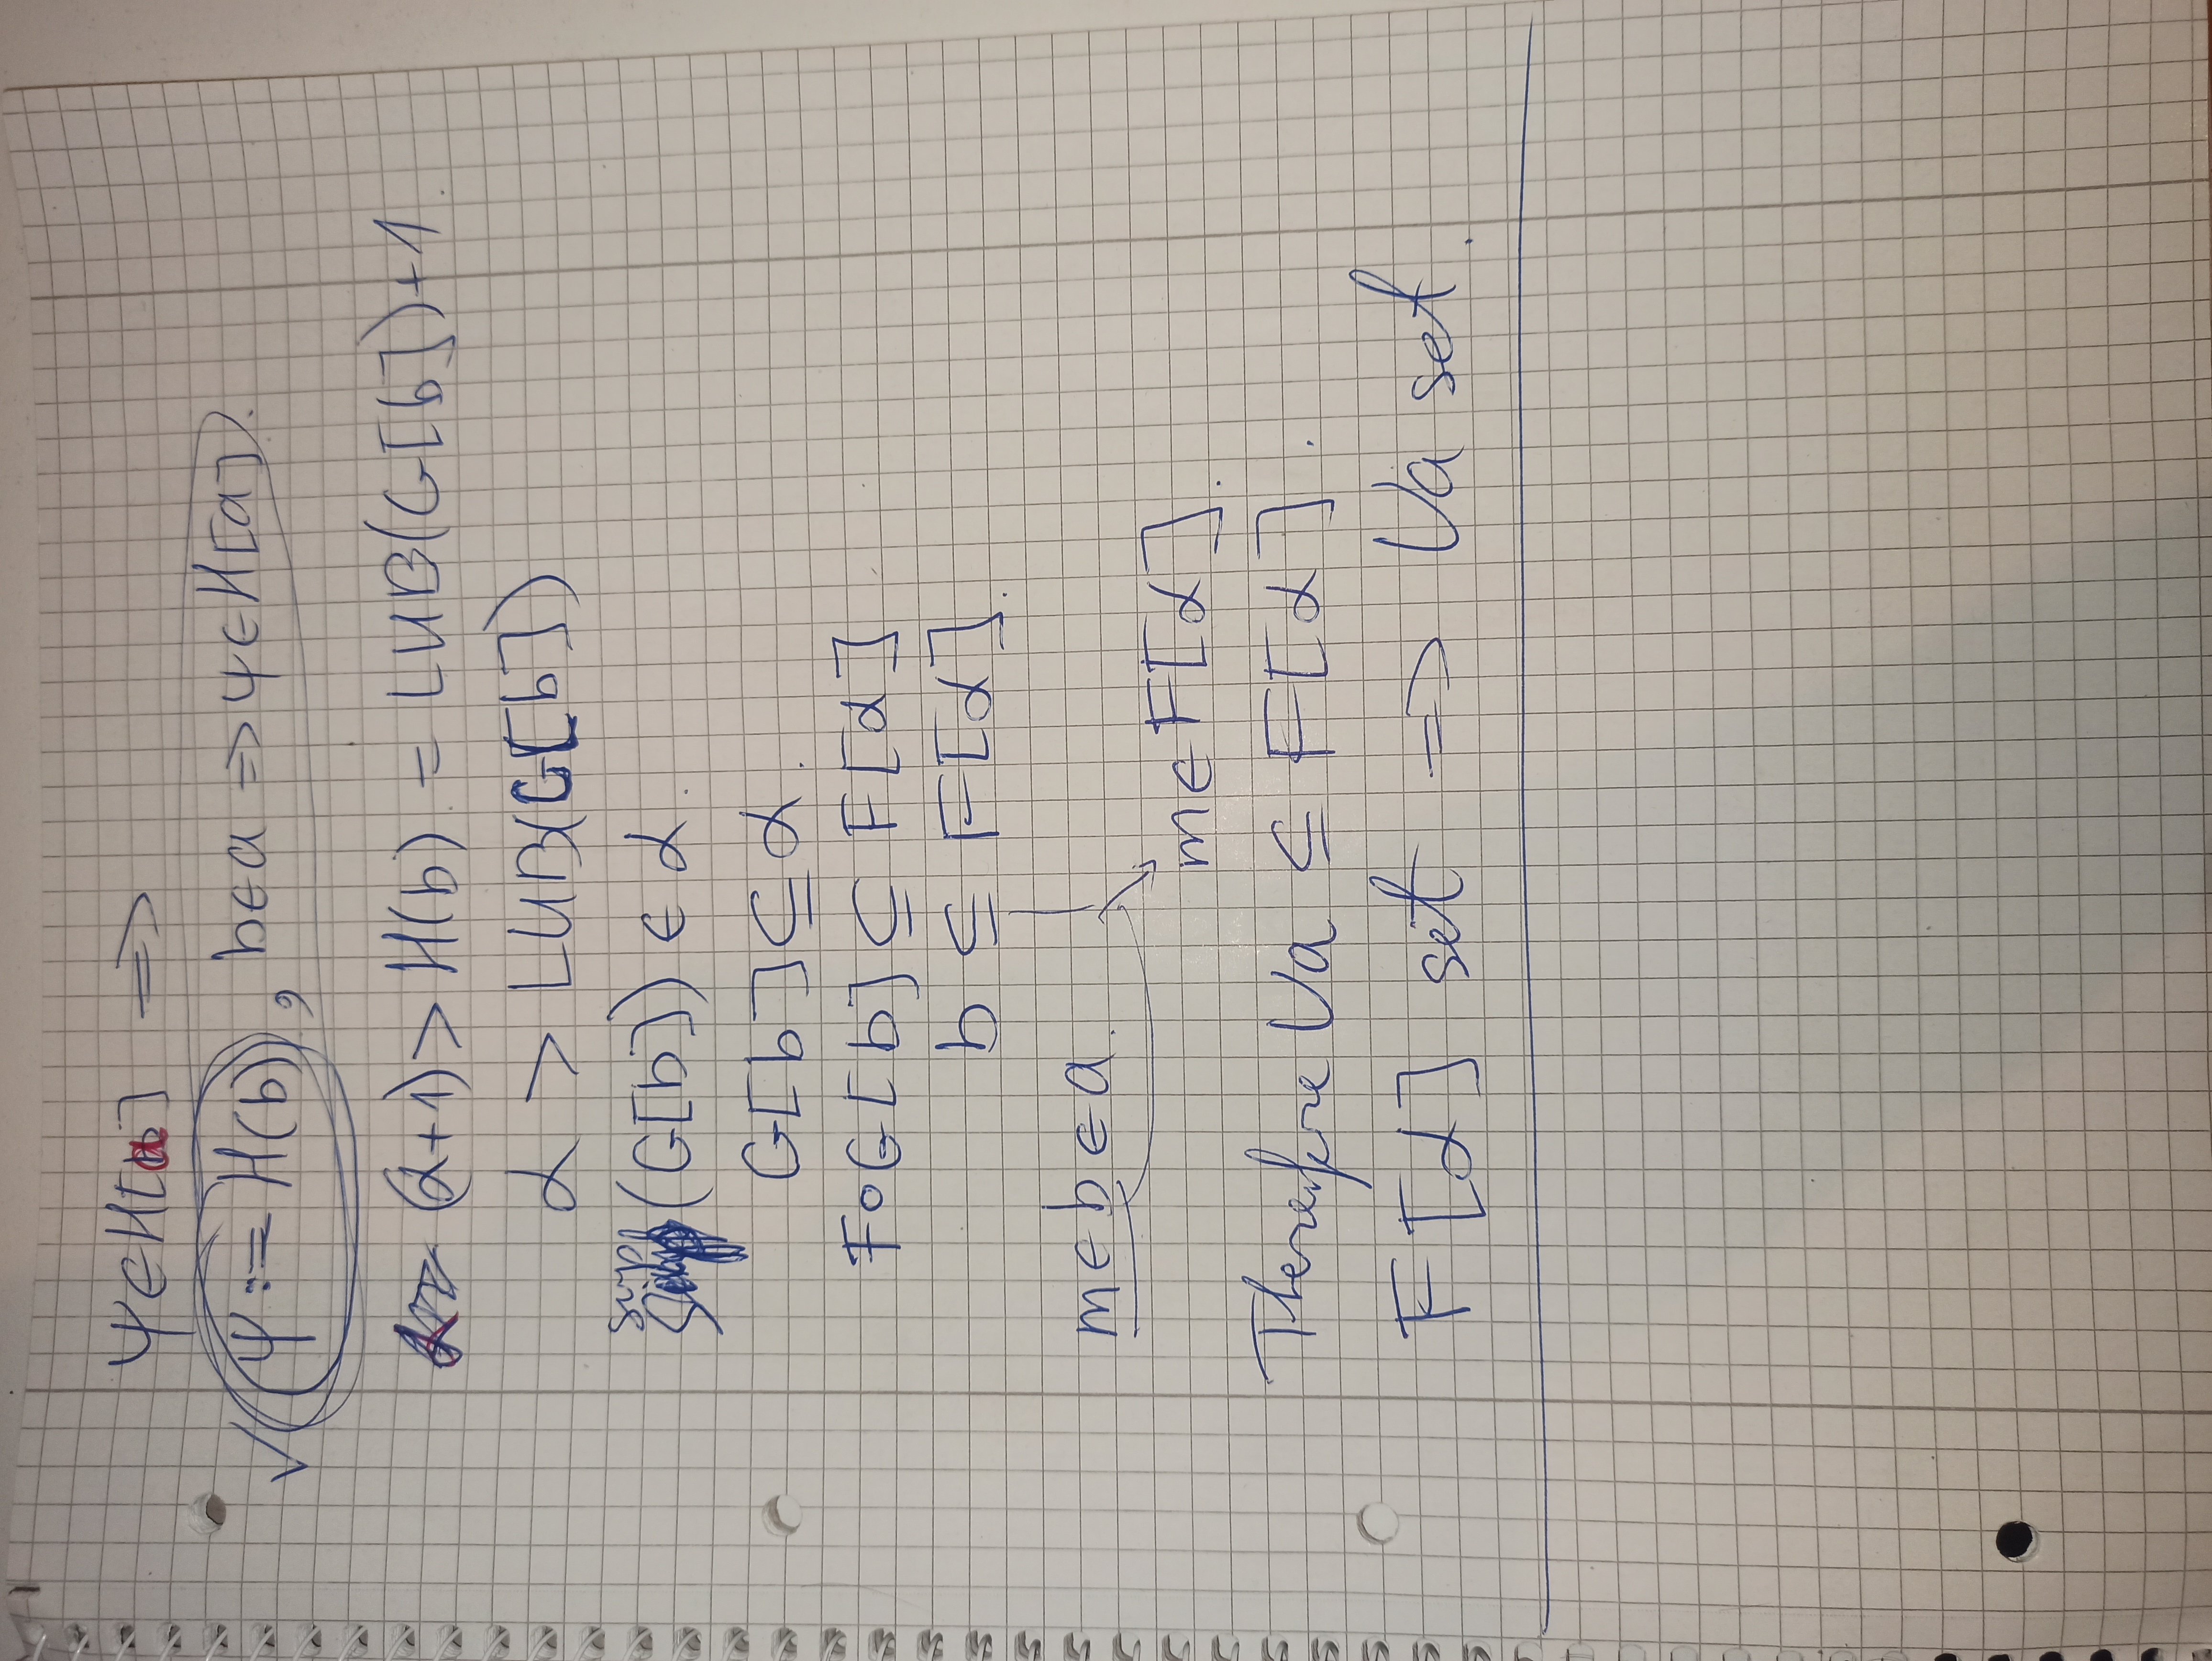
\includegraphics[angle=-90,origin=c,scale=0.1]{azriel_levy/5.jpg}\\
\fi
%\end{document}

\ifdefined\qwertyflag
\undef\qwertyflag
\end{document}
\fi